\chapter{Revisão Bibliográfica} \label{chap:sota}

Neste capítulo é realizada uma revisão bibliográfica das interfaces áudio e vídeo existentes, em específico do HDMI, também sobre métodos de codificação/descodificação de sinais HDMI numa FPGA e ainda sobre ligações de alta velocidade em série e cuidados que se deve ter com as mesmas.

\section{Interfaces de transmissão de video/audio}

As interfaces de áudio e vídeo definem parâmetros físicos e interpretações dos sinais recebidos, segundo \cite{R004}. Para sinais digitais a interface acaba por definir não só a camada física mas também a camada de ligação de dados e principalmente a camada da aplicação. As características físicas do equipamento (elétrico ou ótico) incluem o número e o tipo de ligações necessárias, tensões, frequências, intensidade ótica e ainda o design físico dos conectores. Relativamente à camada de ligação de dados, esta define como os dados da aplicação serão encapsulados para que, por exemplo, possam ser sincronizados ou para fazer correções de erros. Por fim, a camada da aplicação define o formato do sinal de áudio e vídeo a ser transmitido, normalmente incorporando \textit{codecs} não específicos. No entanto, por vezes esta camada acaba por não definir em concreto o tipo de formato de dados deixando em aberto tal parâmetro para que se possa transmitir dados no geral (é o caso do HDMI). No caso dos sinais analógicos, todas as funções que existem para os sinais digitais definidas em três camadas, são representadas num único sinal.

No caso da transmissão de sinais de áudio e vídeo digital existem várias interfaces que passam a ser analisadas, segundo \cite{R004}:
\begin{description}
	\item[$\bullet$  \textbf{\textit{Display Port:}}] utiliza um conector do tipo \textit{DisplayPort} e é o principal concorrente do HDMI. Esta interface define uma interconexão sem licenças que foi inicialmente desenhada para ser utilizada numa conexão entre o computador e o monitor do mesmo. O sinal de vídeo não é compatível com DVI ou HDMI, mas um conector \textit{DisplayPort} pode fazer passar estes sinais.
	\item[$\bullet$   \textbf{\textit{ IEEE 1394 “FireWire":}}] utiliza um conector do tipo \textit{FireWire} ou i.LINK. Este protocolo de transferência de dados é principalmente utilizado em câmaras digitais, mas também em computadores e em transferências de sinal de áudio. Este tipo de interface é capaz de hospedar vários sinais no mesmo cabo entregando os dados nos devidos destinos.
	\item[$\bullet$   \textbf{\textit{HDMI (High Definition Multimedia Interface):}}]utiliza um conector do tipo HDMI e é uma interface de transmissão de sinal áudio/vídeo comprimida para transmissão de sinal digital descomprimida. 
\end{description}

\section{HDMI (\textit{High Definition Multimedia Interface})}\label{sec:dialecto}
O HDMI é uma interface de áudio e vídeo de alta definição que transporta dados áudio no formato não comprimido. Suporta num único cabo qualquer formato de vídeo em diversas resoluções e desde 2004 tem vindo a sofrer algumas alterações que vêm melhorar o desempenho da interface. 

Esta interface está dividida em diversos canais de comunicação que implementam determinados protocolos, entre os quais se destacam as seguintes de \cite{R002}:
\subsection{DDC - \textit{Display Data Channel} } \label{batik} 
É um conjunto de protocolos utilizado nas comunicações digitais entre um dispositvo de origem e um dispositivo final que permite a comunicação entre ambos. Estes protocolos permitem que o ecrã comunique com o seu adaptador quais os modos que consegue suportar e também que o dispositivo que liga ao ecrã consiga ajustar alguns parâmetros, como por exemplo o contraste e a luminosidade. EDID (\textit{Extended display identification data}) é a estrutura \textit{standard} para este tipo de comunicações que define as capacidades do monitor e os modos gráficos suportados pelo mesmo.  Este protocolo é utilizado pela \textit{source} da comunicação do HDMI para obter os dados necessários do dispoistivo \textit{sink}, no sentido de perceber quais os modos suportados pelo mesmo. Este canal é também ativamente usado para HDCP (\textit{High-Bandwith Digital Content Protection}).

\subsection{TMDS - \textit{Transition-Minimized Differential Signaling} } \label{batik} 
É uma tecnologia utilizada para transmissão de dados em série de alta velocidade utilizado em comunicações digitais. O transmissor implementa um algoritmo que reduz as interferências eletromagnéticas nos cabos e permite ainda uma recuperação robusta de sinal de relógio no recetor. 

Em específico na interface HDMI, este protocolo divide a informação a transmitir em 3 principais pacotes e intercala a sua transmissão: Período de transmissão de vídeo, período de transmissão de dados e período de controlo. No primeiro período (período de transmissão de vídeo) são transmitidas os pixeis do vídeo em linha. No segundo período (o período de transmissão de dados) são transmitidos os dados de vídeo e os dados auxiliares à transmissão dentro dos respectivos pacotes. O terceiro período ocorre entre os dois anteriores. 

Para além de ser utilizada no HDMI, esta técnica é também utilizada em interfaces DVI.
\subsection{CEC - \textit{Consumer Electronics Control} } \label{batik} 
É uma característica do HDMI que permite ao utilizador controlar até 15 dispositivos que tenham esta mesma característica ativa e que estão conectados por HDMI usando apenas um controlo remoto. Também é possivel dispositivos inviduais controlarem outros dispositivos sem intervenção do utilizador

\subsection{ARC - \textit{Audio Return Channel}  } \label{batik} 
Esta característica do HDMI utiliza 2 pins do conector. É uma ligação de audio que tem como objetivo substituir outros cabos entre a TV e outros recetores ou então sistema de som. Esta direção é usada quando é a TV que gera ou recebe o vídeo mas é outro equipamente que reproduz o som. Esta característica está apenas disponível a partir da versão 1.4 de HDMI.

\subsection{HEC - \textit{HDMI Ethernet Channel}  } \label{batik} 
Esta especificação do HDMI, tal como a anterior, está também apenas disponível a partir da versão 1.4 do HDMI e é uma tecnologia capaz de consolidar vídeo, audio e dados em série num único cabo HDMI, permitindo também aplicações baseadas em IP sobre o HDMI e uma comunicação \textit{Ethernet} bidireccional até 100 Mbit/s.

Uma das principais características mais recentes das interfaces HDMI prende-se ao facto de permitir que sinais não sejam reproduzidos em dipositivos não autrizados. Isto é, através de um protocolo cujo nome já foi referido anteriormente, HDCP (\textit{High-Bandwith Digital Content Protection}), o sinal HDMI pode ser encriptado e posteriormente transmitido pela \textit{source}, protegendo assim a sua reprodução em dispositivos não autorizados. Esta tem vindo a tornar-se uma característica importante, visto que a reprodução ilegal de vídeos tem vindo a tornar-se reccorrente nos dias atuais.

\section{HDMI implementado sobre a FPGA}
A interface HDMI, tal como descrito no subcapítulo anterior, consiste numa interface que permite a transferência de sinais áudio e vídeo digitais entre dois dispositivos, e como tal será necessário um adaptador que permita a conexão entre os dois dispositivos e que ao mesmo tempo sirva como recurso para a codificação e descodificação do sinal HDMI. 

Assim sendo, existe \textit{hardware} disponível que consegue fazer as duas funções descritas, nomeadamente em \cite{R009}. Esta interface HDMI consiste num adaptador e descodificador do sinal HDMI para a FPGA, sendo que são necessárias uma placa para a transmissão e outra para a receção do sinal. Cada placa tem respetivamente dois transmissores e dois recetores independentes e faz uso dos conectores FMC para se conectar com a FPGA.

\subsection{Conexão à FPGA XILINX VC7203 Virtex-7} \label{batik} 
Na figura~\ref{fig:fpgaVistaGeral} da página~\pageref{fig:fpgaVistaGeral}  visualiza-se a placa de desenvolvimento a ser utilizada no projeto com numeração para as suas diversas características, sendo que nesta fase se pretende perceber o que são os conectores FMC (FPGA Mezzanine Card) e onde estão localizados nesta mesma placa.

\begin{figure}
	\begin{center}
	
		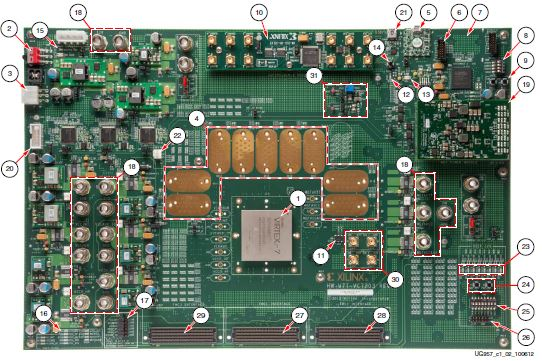
\includegraphics[width=0.86\textwidth]{FPGA}
		\caption{Vista Geral da FPGA VC7203 Virtex-7 retirada de \cite{R008}}
		\label{fig:fpgaVistaGeral}
	\end{center}
\end{figure}